\section{Results}
\label{sec:results}

\subsection{Delaunay triangulation algorithm}
\label{sub:triangulation}

We tested the Bowyer-Watson and Lawson triangulation algorithms for randomly generated inputs of different size.
This is done by recursively adding $n$ points to the initial triangulation.
For each input size, 40 trials were performed.
In Figure \ref{fig:triangulation-runtime} we can see the average time that was needed for inserting the points.
We see that both algorithms don't differ much from each other, but Lawson's triangulation method seems slighty faster than Bowyer-Watsons.

We repeated the same experiments for a constrained triangulation problem.
In addition to the random generated vertices, we now added a PSLG that contrained the way in way the triangulation is performed.
The results are in Figure \ref{fig:triangulation-pslg-runtime}.
Again the difference between the methods is fairly small.

\begin{figure}
    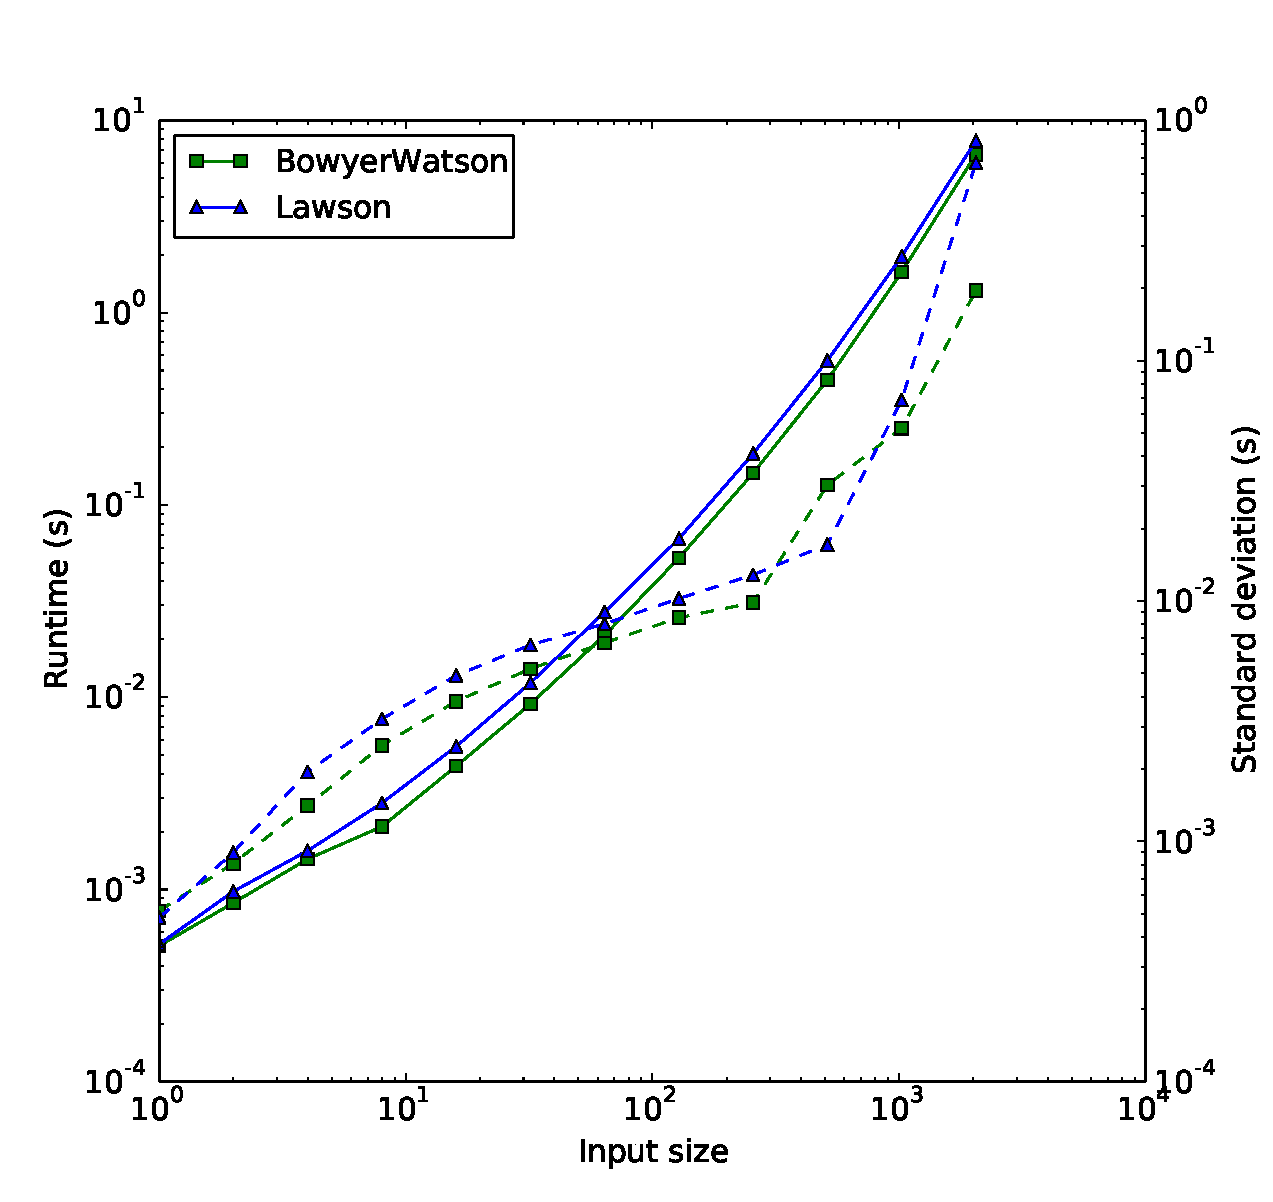
\includegraphics[width=\columnwidth]{../images/runtime.pdf}
    \label{fig:triangulation-runtime}
    \caption{Runtime for triangulation algorithms when input is unconstrained}
\end{figure}

\begin{figure}
    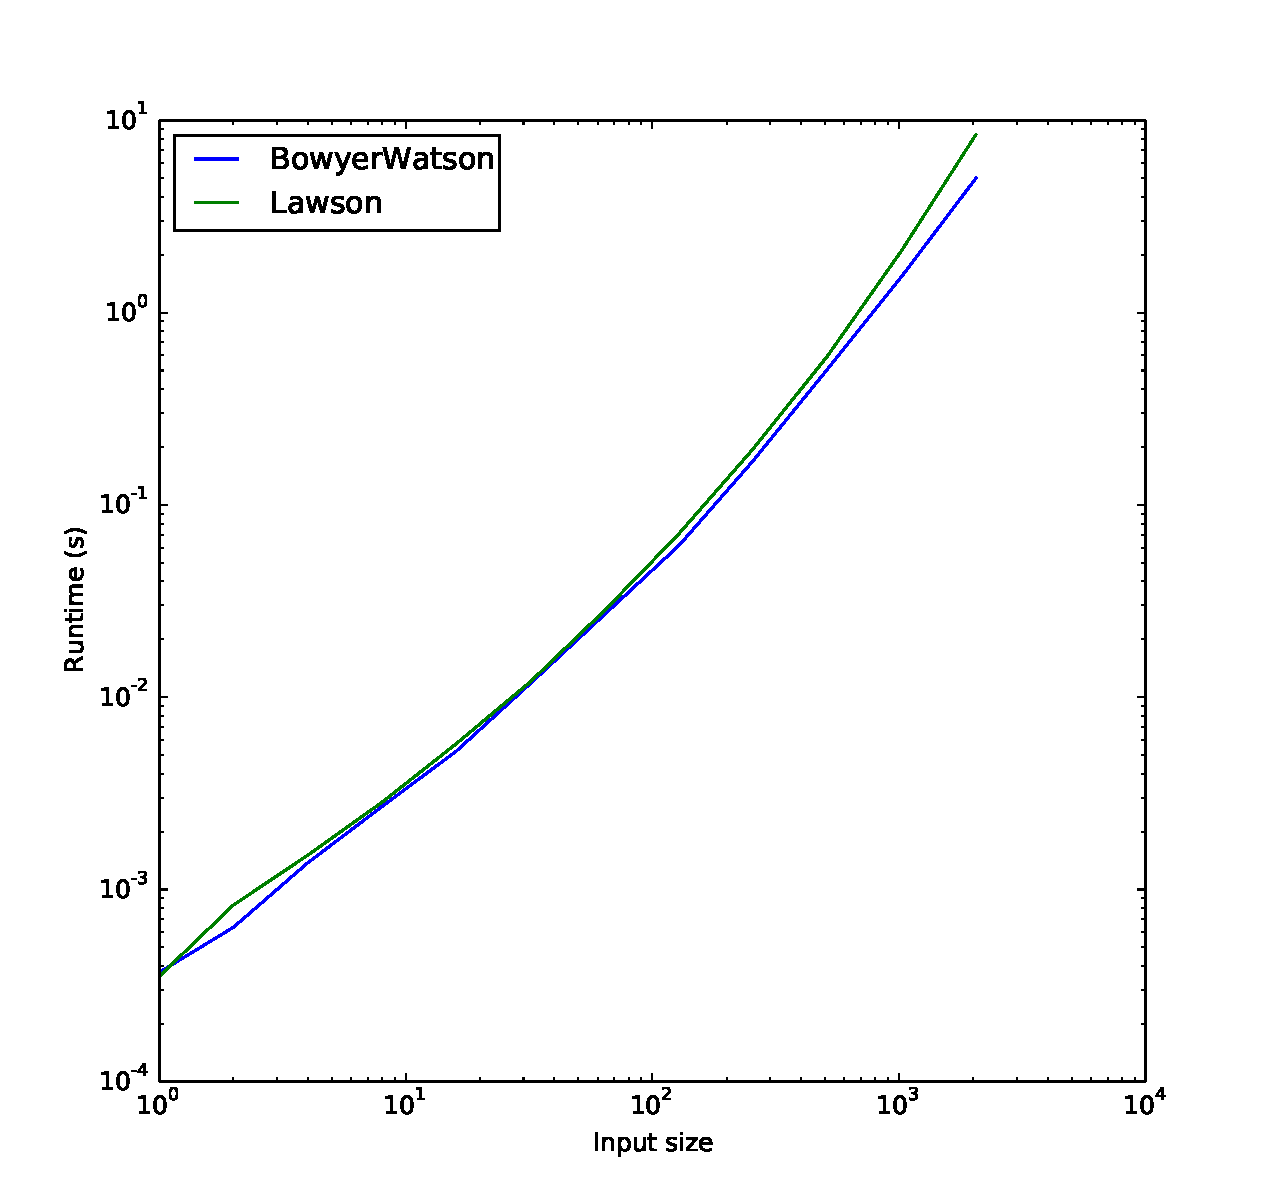
\includegraphics[width=\columnwidth]{../images/runtime_segments.pdf}
    \label{fig:triangulation-pslg-runtime}
    \caption{Runtime for triangulation algorithms when input is constrained by a PSLG}
\end{figure}

\subsection{Ruppert's refinement algorithm}

\begin{figure}
    \centering
    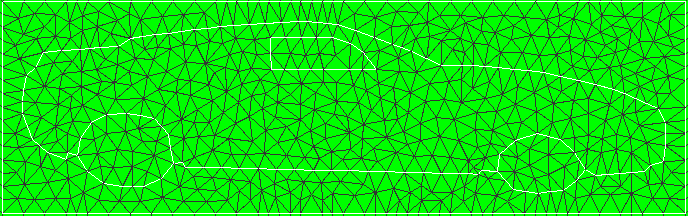
\includegraphics[width=\columnwidth]{../images/Car_Ruppert20.png}
    \caption{Triangulation generated using Ruppert's refinement algorithm for a car. The white lines are PSLG boundary elements.
    The criterea were set to a minimum angle of 20$\degr$ and a maximum area of 200.}
    \label{fig:result_Car20}
\end{figure}

\begin{figure}
    \centering
    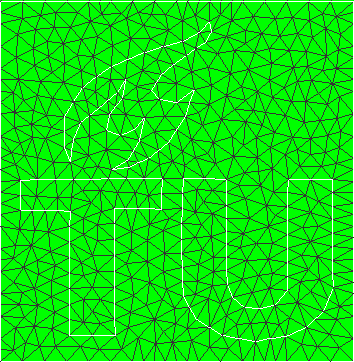
\includegraphics[width=\columnwidth]{../images/TU_Ruppert20.png}
    \caption{Triangulation generated using Ruppert's refinement algorithm for the TU Delft logo. The white lines are PSLG boundary elements.
    The criterea were set to a minimum angle of 20$\degr$ and a maximum area of 200.}
    \label{fig:result_TU20}
\end{figure}
